\documentclass[11pt]{article}

% --- Packages ---
\usepackage[utf8]{inputenc}
\usepackage{amsmath, amssymb, amsthm}
\usepackage{graphicx}
\usepackage{enumitem}
\usepackage[margin=1in]{geometry} 
\usepackage{colortbl} 
\usepackage{array}    
\usepackage{titlesec}
\usepackage{enumitem}
\usepackage{xcolor}
\usepackage[most]{tcolorbox}
\usepackage{listings}
\usepackage{booktabs}
\usepackage{siunitx}
\usepackage{parskip}
\usepackage{float}
\usepackage{caption}
\usepackage{xcolor}
\usepackage{listings}
\usepackage{tabularx}
\usepackage{hyperref}
\usepackage{tikz}
\usepackage{pgfplots}
\pgfplotsset{compat=1.18}


\sisetup{
  group-separator={,},
  group-minimum-digits=4,
  round-mode=places,
  round-precision=2,
  input-ignore={,} % <-- allows commas in input
}

\setlength{\parskip}{6pt}

\setlist[itemize]{label=--}

\setcounter{secnumdepth}{0}

\definecolor{darkblue}{rgb}{0,0,0.8}

\hypersetup{
  colorlinks=true,
  linkcolor=darkblue,
  citecolor=darkblue,
  urlcolor=darkblue
}

\lstset{
  language=Python,
  basicstyle=\ttfamily\small,
  keywordstyle=\color{blue}\bfseries,
  commentstyle=\color{gray},
  stringstyle=\color{orange},
  showstringspaces=false,
  numbers=left,
  numberstyle=\tiny\color{gray},
  breaklines=true,
  frame=single,
  captionpos=b
}

% --- Theorem Environments ---
\theoremstyle{definition}
\newtheorem{definition}{Definition}[section]
\newtheorem{example}{Example}[section]

\theoremstyle{plain}
\newtheorem{theorem}{Theorem}[section]
\newtheorem{lemma}[theorem]{Lemma}

% --- Custom Commands ---
\newcommand{\R}{\mathbb{R}}
\newcommand{\E}{\mathbb{E}}
\newcommand{\Var}{\mathrm{Var}}
\newcommand{\Cov}{\mathrm{Cov}}
\newcommand{\prob}[1]{\mathbb{P}\left(#1\right\)}
\newcommand{\norm}[1]{\left\lVert#1\right\rVert}

\newcommand{\altrowtable}[3]{%
  \renewcommand{\arraystretch}{1.4} 
  \begin{minipage}{0.95\linewidth}
  \rowcolors{1}{gray!10}{white}
  \begin{tabular}{@{} >{\raggedright\arraybackslash}m{#1\linewidth} m{#2\linewidth} @{}}
  #3
  \end{tabular}
  \end{minipage}
}

\lstdefinestyle{rstyle}{
    language=R,
    basicstyle=\ttfamily\footnotesize,
    keywordstyle=\color{blue},
    commentstyle=\color{gray},
    stringstyle=\color{red},
    showstringspaces=false,
    breaklines=true
}

% Box style
\tcbset{
  qa/.style={
    colback=white,
    colframe=black,
    coltitle=black,
    fonttitle=\small\bfseries,
    fontupper=\small,   % �� makes content smaller
    sharp corners,
    boxrule=0.3pt,
    enhanced,
    breakable,
    colbacktitle=white
  }
}

\titlespacing*{\section}{0pt}{*1}{*0.5}
\titlespacing*{\subsection}{0pt}{*0.5}{*0.25}
\setlist{noitemsep, topsep=0pt}

% --- Document Start ---
\begin{document}

% --- Title Page ---
\begin{titlepage}
    \centering
    \vspace*{3cm}
    {\Huge\bfseries MIS 285N: Generative AI I \par}
    \vspace{1.5cm}
    {\Large Gabriel Kinshuk \par}
    \vspace{0.5cm}
    {\large Instructor: Dr. Constantine Caramanis \par}
    \vfill
    {\large Spring 2026 \par}
\end{titlepage}

% --- Table of Contents ---
\tableofcontents
\clearpage

\newpage
\section{Neural Networks}

\bigskip

\subsection{Fully Connected Linear Layers}

\medskip

Also called a \textit{dense} layer, is a layer where every input neuron is connected to every output neuron. Then, for an input vector $x$, bias vector $b$, and weight matrix $A$, the output $y$ is simply calculated as:
\[
y = xA^T + b
\]
Which is an \textit{affine} transformation (a linear transformation followed by a translation). The number of trainable parameters at this layer is equal to the number ($n$) of edges between the input neurons and output neurons, plus the biases:
\begin{center}
    Trainable parameters = $n_{in} \times n_{out} + n_{out}$
\end{center}

\subsubsection{Activation Functions}

By itself, a sequence of linear layers is mathematically equivalent to a single linear layer. To learn non-linear patterns, the output $y$ is typically passed through an \textit{activation function} $\sigma$ (such as ReLU or Sigmoid):
\[
z = \sigma(xA^T + b)
\]

\medskip

\begin{table}[H]
\centering
\renewcommand{\arraystretch}{1.5}
\rowcolors{2}{gray!10}{white}
\begin{tabularx}{0.95\textwidth}{l l X}
\toprule
\textit{Function} 
& \textit{Equation} 
& \textit{Notes} \\
\midrule
ReLU 
& $f(x) = \max(0, x)$ 
& Standard for hidden layers. Efficient and reduces vanishing gradients, but can suffer from "dying neurons" where nodes become permanently inactive. \\

Leaky ReLU 
& $f(x) = \max(\alpha x, x)$ 
& Addresses the dying ReLU problem by allowing a small, non-zero gradient $\alpha$ (e.g., $0.01$) for negative inputs. \\

Sigmoid 
& $\sigma(x) = \frac{1}{1 + e^{-x}}$ 
& Squashes values to the range $(0, 1)$. Primarily used for binary classification outputs; prone to vanishing gradients in deep layers. \\

Tanh 
& $\tanh(x) = \frac{e^x - e^{-x}}{e^x + e^{-x}}$ 
& Zero-centered output in the range $(-1, 1)$. Generally leads to faster convergence than sigmoid but remains susceptible to vanishing gradients. \\
\bottomrule
\end{tabularx}
\caption*{Summary of common activation functions used in neural networks.}
\end{table}

\subsubsection{Universal Approximation Theorem}

The non-linearity of the activation function allows the network to approximate any continuous function, a property known as the \textit{Universal Approximation Theorem}. We can think of this similar to a Riemann sum, where each neuron creates a piecewise linear approximation of a larger curve. As the width of the hidden layer increases, the interval becomes smaller (and the resolution of the approximation improves). 

Although the theorem states that for any given problem, a perfect approximation exists, there is no guarantee that gradient descent will find the perfect parameters that define that approximation. Additionally, in practice it is more parameter-efficient to approximate complex functions using deep layers rather than a single wide one.

\medskip

\subsubsection{The Output Layer}

While we are often afforded significant flexibility in the hidden layer dimensionality, the final output layer's dimension is highly dependent on the task. For a regression, there is typically a single output neuron with no activation. For a classification, there are as many output neurons as there are classes (except for binary classification, in which we can use a single neuron with a sigmoid activation). These outputs are called \textit{logits} (or log-odds), which can be processed through a softmax layer (normalized exponential) to convert them into probabilities for each class that sum to 1:
\[
\text{Softmax}(z_i) = \frac{e^{z_i}}{\sum_{j=1}^{n} e^{z_j}}
\]

\subsubsection{The Input Layer}

Although it is described as an ``input layer", it is not a layer of neurons performing a calculation. Therefore, there are no parameters like weights or biases with it. When drawing a network, we may attribute the edges as weights belonging to the input layer, but those weights actually belong to the ``receiving" nodes in the subsequent layer. 

A final note is that if the input is a tensor (multi-dimensional matrix), such as for images, the data must be flattened into a one-dimensional vector before entering the linear layer. In modern deep learning frameworks, input tensors typically include a \textit{batch dimension} $N$, which represents the number of samples processed in parallel. 

The flattening operation is applied only to the spatial/feature dimensions, while the batch dimension remains untouched to ensure each sample is processed independently. For a typical image tensor:
\[
X \in \mathbb{R}^{N \times C \times H \times W} \xrightarrow{\text{flatten}} X_{flat} \in \mathbb{R}^{N \times d}, \quad \text{where } d = C \times H \times W
\]

The resulting matrix dimensions must align with the weight matrix $A \in \mathbb{R}^{n_{out} \times d}$.

\bigskip

\subsection{Introduction to Gradient Descent}

\medskip

Since the error surface for neural networks is often complex and non-convex, no closed-form solution exists to solve for the weights directly. Weights are updated iteratively by calculating the current error and finding the \textit{gradient}, which is the vector of partial derivatives with respect to each weight $\theta$. We take a step in the direction of the negative gradient to minimize the loss.

We define a loss function $L(\theta)$ to quantify error. The Mean Squared Error (MSE) is a common choice where $y$ is the target and $f_\theta(x)$ is the model prediction:

$$L(\theta) = \frac{1}{n} \sum_{i=1}^n (y_i - f_\theta(x_i))^2$$

In a non-convex landscape, the negative gradient points toward the steepest local decline. This can lead the model to get stuck in local minima or at saddle points. Strategies such as momentum, adaptive learning rates (like Adam), and mini-batch randomization are used to help the algorithm navigate these features and find a better global solution. An example of this calculating a gradient descent step is \hyperref[worked-gradient-descent]{here}.

Gradient descent has limitations. For one, it depends entirely on the error surface, which itself is a function of the weights. If our choice of weights and features is insufficient for the problem, then we can never come up with a good solution. Consider the following data matrix and target vector for the XOR function:

\[
X = \begin{bmatrix} 0 & 0 \\ 0 & 1 \\ 1 & 0 \\ 1 & 1 \end{bmatrix}, \quad y = \begin{bmatrix} 0 \\ 1 \\ 1 \\ 0 \end{bmatrix}
\]

There does not exist a set of weights for a purely linear layer that can solve the problem, because the problem itself is nonlinear. Using ReLU, we can create a model with 0 training error, seen \hyperref[worked-XOR-relu-model]{here}.

\bigskip

\subsection{Code Implementation with PyTorch}

\medskip

\noindent
\begin{minipage}[t]{0.55\textwidth}
\vspace{0pt}

\begin{lstlisting}[language=Python]
import torch
import torch.nn as nn

class MyNNet(nn.Module):
    def __init__(self):
        super(MyNNet, self).__init__()
        self.fc1 = nn.Linear(2, 2)
        self.fc2 = nn.Linear(2, 1)
        self.relu = nn.ReLU()

    def forward(self, x):
        x = self.fc1(x)
        x = self.relu(x)
        x = self.fc2(x)
        return x

model = MyNNet()
\end{lstlisting}

\end{minipage}
\hspace{1em}
\begin{minipage}[t]{0.4\textwidth}
\vspace{0pt}

\textbf{Layer details}

\begin{itemize}
\item The output dimension of \texttt{fc1} must match the input dimension of \texttt{fc2}.  
      Here both are $2$, so the hidden representation has width $2$.

\item \texttt{nn.Linear(in, out)} automatically includes a bias term, so each layer learns both weights and offsets.

\item \texttt{ReLU} is applied elementwise to the 2-dimensional hidden vector.

\item The final layer has no activation. 
\end{itemize}

\end{minipage}

\medskip

\textbf{Why define \texttt{forward}?}

In PyTorch, the \texttt{forward} method explicitly specifies how data flows through the network. When we call \texttt{model(x)}, PyTorch executes \texttt{forward(x)} and constructs a \emph{computation graph}, which is a record of the operations applied to the input and how they depend on one another. Each layer and activation becomes a node in this graph. During backpropagation, PyTorch follows this same graph in reverse to compute gradients using the chain rule. Some high-level TensorFlow APIs hide this step by assuming a fixed layer sequence, but PyTorch requires the forward pass to be written explicitly so the architecture is fully transparent.

\bigskip



\section{Convolutional Neural Networks}

\medskip

Unlike tabular data, images have spatial structure. Nearby pixels are related, and meaningful patterns such as edges, textures, or object parts appear locally. A fully connected network ignores this structure and treats every pixel independently.

In a fully connected layer, every hidden neuron receives input from every pixel. If the input has $n$ features and the hidden layer has $m$ neurons, the layer learns $n \times m$ weights. As images grow larger, this quickly becomes impractical. More importantly, the model does not respect locality. A pixel in one corner of the image is treated no differently from a pixel in the center.

Convolutional Neural Networks (CNNs) impose two structural constraints: local connectivity and weight sharing. Each neuron only looks at a small window of the input rather than the entire image. For example, a $3 \times 3$ filter examines only nine neighboring pixels at a time. This reflects the fact that useful visual patterns are local. The small matrix of learnable weights that defines a filter is called the \textit{kernel}. Since we apply the kernel elementwise and take the sum, the neuron activation will be highest over a region that most ``looks like" the kernel. 

The second idea is weight sharing. The same set of filter weights is reused at every spatial location. Although a convolutional layer may produce many output neurons, they do not each learn independent parameters. If a filter has $k$ parameters, then the entire layer uses those same $k$ parameters everywhere it is applied. The filter slides across the image, but its weights remain fixed.

These constraints dramatically reduce the number of parameters and encode an important prior: patterns such as edges or textures can appear anywhere in the image. A convolutional layer therefore learns what pattern to detect, not where it occurs.

\bigskip

\subsection{Multiple Channels}

\medskip

So far we have treated a convolution as a single 2D filter producing one feature map. Real images, however, have multiple channels. An RGB image has three channels, so a filter must span all of them. Instead of an $M \times M$ matrix, each filter is an $M \times M \times 3$ tensor. The spatial footprint is still local, but the filter now combines information across color channels at every location.

Moreover, we typically learn not just one filter, but many. Each filter produces its own feature map, and these maps are stacked along a new channel dimension. This is how a layer can detect multiple types of patterns simultaneously.

\medskip

In PyTorch, this is specified as

\[
\texttt{nn.Conv2d(in\_channels, out\_channels, kernel\_size, stride, padding)}.
\]

\begin{itemize}[itemsep=0.3em]
\item \texttt{in\_channels}: Number of input channels. For an RGB image, this is 3. In deeper layers, it equals the number of feature maps from the previous layer.

\item \texttt{out\_channels}: Number of filters the layer learns. Each filter produces one output feature map.

\item \texttt{kernel\_size}: Spatial size of the filter (e.g., $3$ for a $3 \times 3$ kernel).

\item \texttt{stride}: Step size of the filter as it moves across the image. Larger stride reduces spatial resolution.

\item \texttt{padding}: Number of pixels added around the border of the input (typically zeros), which controls whether spatial dimensions shrink or are preserved.
\end{itemize}

Together, these arguments determine both how many pattern detectors the layer learns and how the spatial dimensions evolve from one layer to the next.

\subsection{Counting Parameters and Output Size}

\medskip

\textbf{Number of weights in a convolutional layer.}

For a convolutional layer defined as
\[
\texttt{nn.Conv2d}(C_{\text{in}}, C_{\text{out}}, K, s, p),
\]
the total number of learnable weights is

\[
n_{\text{weights}}
=
C_{\text{out}}
\times
C_{\text{in}}
\times
K
\times
K.
\]

If a bias term is used (default in PyTorch), then we add $+ \; C_{\text{out}}$.

\medskip

As a note, stride $s$ and padding $p$ do \textit{not} affect the number of parameters, because they change how many times the filter is applied and the spatial size of the output, but the same weights are reused at every location.

\bigskip

\textbf{Output spatial size of the next layer.}

If the input has spatial size $H \times W$, kernel size $K$, stride $s$, and padding $p$, then the output height and width are

\[
H_{\text{out}}
=
\left\lfloor
\frac{H - K + 2p}{s}
\right\rfloor
+ 1,
\qquad
W_{\text{out}}
=
\left\lfloor
\frac{W - K + 2p}{s}
\right\rfloor
+ 1.
\]

\begin{itemize}[label=$\circ$, itemsep=0.3em]
\item $H - K$: once a $K \times K$ filter is placed on the image, it cannot extend past the boundary. Subtracting $K$ accounts for the size of the window.

\item $+\,2p$: padding adds $p$ pixels on both sides of the image, effectively increasing the usable spatial dimension by $2p$.

\item $\div\, s$: stride determines how far the filter moves each step. Dividing by $s$ counts how many valid positions the filter can occupy.

\item $+\,1$: accounts for the initial placement of the filter at the first valid position.
\end{itemize}

The floor function ensures the result is an integer if the division is not exact.  
The number of output channels is simply $C_{\text{out}}$, since each learned filter produces one output feature map.  

Therefore, the full output volume has shape
$H_{\text{out}} \times W_{\text{out}} \times C_{\text{out}}$.

If we really want to be pedantic, in PyTorch, tensors are stored in the order $(\text{batch size},\, C_{\text{out}},\, H_{\text{out}},\, W_{\text{out}})$.

\medskip

Lastly, we can consider \textit{pooling layer}. Pooling layers reduce spatial resolution without introducing additional learnable parameters. Instead of learning weights, they apply a fixed operation over local windows. Max pooling keeps the strongest activation in each region, emphasizing the most prominent feature, while average pooling smooths the region by taking the mean value. In both cases, the spatial dimensions shrink, which lowers computational cost and makes the representation more robust to small translations in the input.

If we wanted to implement average pooling in a \textit{forward} function, we could add the line \texttt{x = x.mean(dim=(2,3))}, where 2 and 3 are the height and width dimensions in the input tensor.

\bigskip



\section{Logistic Regression}

\medskip

Logistic regression can be viewed as the simplest neural network: a model with no hidden layers and a single linear transformation feeding directly into a probabilistic output. In this sense, it is a one-layer neural network trained with cross-entropy loss.

It learns a linear decision boundary by assuming that the log-odds of the two classes are a linear function of the input. When the data are not perfectly linearly separable, different loss functions produce different separating hyperplanes, even though the classifier itself remains linear.

\bigskip

\subsection{Measuring Loss}

\medskip

Consider data in $\mathbb{R}^2$ where $x_1$ is informative and $x_2$ is mostly noise. As we slide a linear decision boundary along the $x_1$ axis, we can evaluate its quality using different loss functions.

The most direct measure is the classification error rate. However, as a function of the boundary location, the error rate is \emph{discontinuous}. A small change in the boundary does nothing until it crosses a data point, at which point the loss jumps. This makes optimization difficult: gradients do not exist, and one would need to search explicitly, leading to slow convergence on the order of $\mathcal{O}(1/\epsilon)$ to reach accuracy $\epsilon$.

Instead, we use smooth surrogate losses such as hinge loss, exponential loss, or cross-entropy loss. These are convex and differentiable, which allows efficient gradient-based optimization. For convex losses, convergence to accuracy $\epsilon$ can occur in time on the order of $\mathcal{O}(\log(1/\epsilon))$ under standard assumptions.

Cross-entropy loss differs from minimizing classification error directly. Rather than penalizing only misclassifications, it penalizes \emph{confidence}. Predictions that are correct but uncertain still incur loss, and incorrect predictions that are confident incur large loss. This produces a smoother optimization landscape and leads to probabilistic outputs instead of just hard decisions.

In non-separable data, cross-entropy does not attempt to eliminate every classification error. Instead, it adjusts the boundary to reduce the total loss over all points. If correcting a small cluster would increase the loss on a much larger group, the optimizer will leave that cluster misclassified. The solution is determined by the aggregate contribution of all data points to the objective.

At the same time, points that lie near the decision boundary receive probabilities close to $0.5$ for each class, meaning the model has low confidence. If such a point is misclassified, the cross-entropy loss is moderate rather than large, because the prediction was not confident. For example, if the model distinguishes only red and blue but a point lies in a region that is effectively ambiguous between them, the best it can do is assign intermediate probabilities (approximately $0.5, 0.5$). The boundary may shift so that ambiguous regions correspond to uncertain predictions rather than confident errors.

\bigskip

\subsection{Convex Functions}

\medskip

A function $f$ is called \emph{convex} if, for any two points $x_1, x_2$ in its domain, the line segment joining $(x_1, f(x_1))$ and $(x_2, f(x_2))$ lies above the graph of the function. Analytically, this means that for any $\lambda \in [0,1]$,

\[
f\big(\lambda x_1 + (1-\lambda)x_2\big)
\;\le\;
\lambda f(x_1) + (1-\lambda) f(x_2).
\]
The left-hand side evaluates the function at a convex combination of the inputs.  
The right-hand side forms the same convex combination of the function values.  

Convexity therefore guarantees that averaging inputs cannot produce a function value larger than averaging the outputs. Another key characteristic of convex functions are that any local optimum must also be the \textit{global} optimum. 

\bigskip

\subsection{Gradient Descent}

\medskip

We defined the loss as
\[
L(\theta) = \frac{1}{n}\sum_{i=1}^n \text{Loss}(x_i, \theta),
\]
so its gradient is

\[
\nabla L(\theta)
=
\sum_{i=1}^n \nabla \text{Loss}(x_i, \theta).
\]

The full-batch update therefore takes the form
\[
\theta_{t+1}
=
\theta_t
-
\eta
\sum_{i=1}^n
\nabla \text{Loss}(x_i, \theta_t).
\]

For large datasets, evaluating this sum at every step is costly.  
Instead, we approximate it using a subset $S \subset \{1,\dots,n\}$:

\[
\theta_{t+1}
=
\theta_t
-
\eta
\sum_{i \in S}
\nabla \text{Loss}(x_i, \theta_t).
\]

If $|S|=1$, this is stochastic gradient descent.  
If $1<|S|<n$, this is mini-batch gradient descent.  
Mini-batching reduces computation per update and injects useful noise into the optimization process.

\medskip

In PyTorch, the \texttt{DataLoader} handles mini-batching.  
Within the training loop,

\begin{itemize}
\item \texttt{loss.backward()} computes the gradient of the batch loss,
\item \texttt{optimizer.step()} updates the parameters via
\[
\theta \leftarrow \theta - \eta\,\widehat{\nabla L(\theta)},
\]
\end{itemize}

where $\widehat{\nabla L(\theta)}$ denotes the gradient evaluated on the current batch.  
With the default mean reduction, this is the average of the per-sample gradients in that batch.

Each call to \texttt{optimizer.step()} therefore performs one gradient descent update based only on the selected subset of data.

\bigskip

\subsection{Code Implementation with PyTorch}

\medskip

\noindent
\begin{minipage}[t]{0.55\textwidth}
\vspace{0pt}

\begin{lstlisting}[language=Python]
import torch
import torch.nn as nn

class SimpleLogisticNN(nn.Module):
    def __init__(self):
        super(SimpleLogisticNN, self).__init__()
        self.linear = nn.Linear(2, 2)

    def forward(self, x):
        x = self.linear(x)
        x = nn.functional.softmax(x, dim=1)
        return x

model = MyNNet()
\end{lstlisting}

\end{minipage}
\hspace{1em}
\begin{minipage}[t]{0.4\textwidth}
\vspace{0pt}
\raggedright

\texttt{nn.Linear(2,2)} defines a single linear layer mapping 2 input features to 2 output logits.

\medskip

\texttt{nn.functional.softmax} applies the softmax activation. The \texttt{nn.functional} module contains stateless activation functions that are applied directly in the forward pass.

\medskip

\texttt{dim=1} specifies that softmax is computed across the class dimension (the second axis of the tensor), so each row of the batch is converted into a probability distribution.

\end{minipage}

\bigskip

\subsection{Geometric Interpretation of Logistic Regression}

\medskip

Logistic regression is fundamentally a geometric model.  
Each class has an associated weight vector $w$, and the model computes the inner product
\[
z = w^\top x.
\]
This inner product measures how aligned the input vector $x$ is with the weight vector $w$.

\medskip

Geometrically, the inner product can be written as
\[
w^\top x = \|w\|\,\|x\|\cos\theta,
\]
where $\theta$ is the angle between the two vectors.  
If $x$ points in roughly the same direction as $w$, the cosine is positive and large.  
If it points in the opposite direction, the cosine is negative.  
Thus, logistic regression classifies points based on their alignment with the learned weight vectors.

\medskip

In the multi-class case, each class has its own weight vector $w_k$, producing logits
\[
z_k = w_k^\top x.
\]
The softmax function then converts these scores into probabilities.  
The predicted class is the one whose weight vector has the largest inner product with $x$.

\medskip

The decision boundary between two classes occurs when their scores are equal:
\[
w_1^\top x = w_2^\top x.
\]
Rewriting,
\[
(w_1 - w_2)^\top x = 0,
\]
which defines a hyperplane.  

Therefore, logistic regression separates space with linear hyperplanes, and classification depends on which weight vector is most aligned with the input.



\bigskip



\section{Transfer Learning}

\medskip

Training large neural networks from scratch requires enormous amounts of data and computation. Transfer learning addresses this by reusing representations learned in one domain and applying them to another.

The basic idea is simple, first we train a large network on a huge dataset, then reuse the learned representations for a different but related task. In practice, we typically replace the final output head to match the new objective (e.g., regression instead of classification, or a different number of classes). Initially, we may freeze the earlier layers and train only this new head. After it stabilizes, we can optionally unfreeze some or all of the earlier layers and fine-tune the network so that the shared features become better specialized to our dataset.

\medskip

Early layers of deep networks tend to learn general features such as edges, textures, and simple shapes.  
These low-level patterns appear across many image domains. Later layers become task-specific. If the new task is related to the original one, the earlier representations remain useful. We only need to adapt the final layers.

\medskip

Transfer learning works best when the source and target domains share structure.  If the new dataset is small but related to the original dataset, the pre-trained features provide a strong starting point. For example, even though ImageNet consists of natural images and ultrasound images look very different, low-level visual patterns such as edges and textures are still present. The network can reuse these early features and adapt the higher-level layers to the new medical task.

\bigskip



\section{Embeddings}

\medskip

Recall that in logistic regression the score for a class is an inner product, $z = \langle W, X \rangle.$. Geometrically, this quantity is large when the vectors $W$ and $X$ are aligned, that is, when the angle between them is small. On the unit sphere,
\[
\langle W, X \rangle = \|W\| \|X\| \cos \theta,
\]
so classification reduces to measuring geometric similarity. This geometric view becomes much more powerful in deep networks. Suppose we take an input vector
\[
X = [x_1, x_2, \dots, x_n]^T
\]
and pass it through multiple layers: convolution, ReLU, pooling, fully connected layers. The output of these transformations is a new vector
\[
h = f_\theta(X),
\]
which is another numerical representation of the same data. This vector $h$ is called an \emph{embedding}.

\begin{itemize}
\item In the original input space (for example, raw pixel space), classes may be highly intertwined.
\item After applying a learned nonlinear transformation, the data are mapped into an embedding space.
\item In this embedding space, the classes are often close to linearly separable.
\end{itemize}

The final layer of a neural network is typically just logistic regression applied to this embedding:
\[
z_k = \langle W_k, h \rangle,
\qquad
y = \text{softmax}(z).
\]
In other words, the network first learns a representation where geometry reflects semantic similarity, and then applies a linear classifier in that space.

\bigskip

\subsection{Why this matters}

\medskip

Consider logistic regression applied directly to CIFAR-10 cats and dogs in pixel space.  
The accuracy remains low because the two classes are not linearly separable in raw pixel coordinates. If they were, a linear model would achieve low loss and high accuracy.

Now consider a pre-trained network such as ResNet18.  
If we remove the final classification layer and extract the penultimate layer activations, we obtain an embedding vector for each image. When these embeddings are projected into two dimensions, we observe that cats and dogs are nearly separable by a linear boundary, thus the representation has changed the geometry of the data.

\bigskip

\subsection{Geometric distance vs. semantic distance}

\medskip

In raw pixel space, two images of kangaroos can be extremely far apart numerically. Pixel-by-pixel they may differ in lighting, background, orientation, and scale. Geometrically, they are distant, yet semantically they are very similar.

A good embedding replaces pixel-level distance with a learned geometric distance that reflects meaning. Images that depict the same concept are mapped to nearby points in embedding space. Images of different concepts are pushed farther apart. Thus, embeddings convert semantic similarity into geometric proximity.

\bigskip

\subsection{General perspective}

\medskip

Embeddings are not limited to images. The same idea applies to words, text, audio, or even multimodal combinations of images and language. In each case, the goal is the same: learn a transformation
\[
X \mapsto h
\]
such that simple geometric operations in the embedding space, such as inner products or linear separators, solve tasks that are highly nonlinear in the original space. From this perspective, a deep network can be viewed as:

\begin{enumerate}
\item A feature extractor that constructs an embedding where the data are organized geometrically by meaning.
\item A final linear classifier that separates the classes in that embedding space.
\end{enumerate}

\bigskip

\subsection{Search/Retrieval}

\medskip

Embeddings fundamentally change how we perform search and retrieval. Exact string matching is brittle: if we search for `bicycle' using \texttt{ctrl-f}, we will miss occurrences of `bike', `cycling', or `two-wheeler'. Even with heuristic normalization rules such as stemming or lemmatization, exact matching only captures surface-level variations of the same token. It does not capture semantic equivalence or relatedness. What we actually want is retrieval based on meaning rather than spelling.

As discussed earlier, each word $w$ is mapped to a vector $v_w \in \mathbb{R}^d$ such that semantic similarity corresponds to geometric proximity in embedding space. In particular, the angle $\theta_{\alpha\beta}$ between $v_\alpha$ and $v_\beta$ should be small when the meanings of $\alpha$ and $\beta$ are similar. Therefore, instead of matching strings, we rank documents by cosine similarity:
\[
\cos(\theta_{\alpha\beta}) 
=
\frac{\langle v_\alpha, v_\beta \rangle}
{\|v_\alpha\|\,\|v_\beta\|}.
\]

The normalization by $\|v_\alpha\|\,\|v_\beta\|$ is necessary because embeddings are not constrained to have unit norm. Cosine similarity removes dependence on vector magnitude and isolates angular similarity, which is what encodes semantic relatedness.

\medskip

This reframes search as a nearest-neighbor problem in $\mathbb{R}^d$. Given a query word or phrase embedding $v_q$, we retrieve items whose embeddings have the largest inner product or cosine similarity with $v_q$.

\bigskip

\subsubsection{Self-Supervision and Learning Embeddings}

\medskip

We now address the central question: how do we learn these vectors?

Suppose our dictionary contains $30{,}000$ words. There are roughly $9 \times 10^8$ ordered word pairs. It is infeasible to manually specify a target similarity or angle $\theta_{\alpha\beta}$ for every pair. Even if such targets were available, directly solving for vectors satisfying
\[
\angle(v_\alpha, v_\beta) \approx \theta_{\alpha\beta}
\quad \text{for all } (\alpha,\beta)
\]
would be computationally and statistically intractable.

\medskip

The key idea is \emph{self-supervision}. We exploit an essentially inexhaustible resource: raw text. Instead of hand-labeling semantic relationships, we construct a supervised learning problem from the text itself. Recall that in supervised learning we observe labeled examples
\[
(X_1, y_1), (X_2, y_2), \dots, (X_n, y_n),
\]
and we learn a function $f_\theta$ mapping $X \mapsto y$. Our original objective is to learn semantic embeddings. To use the machinery of supervised learning, we must cast this goal into the form of labeled examples $(X,y)$. We do this by predicting word co-occurrence.

Consider a corpus containing the text:
\begin{quote}
``April is the cruelest month, breeding lilacs out of the dead land, mixing memory and desire, stirring dull roots with spring rain.''
\end{quote}

From this corpus, we can automatically generate training examples such as:
\[
X_1 = (\text{April}, \text{cruelest}), 
\quad 
y_1 = P(\text{cruelest follows April}),
\]
\[
X_2 = (\text{breeding}, \text{lilacs}), 
\quad 
y_2 = P(\text{lilacs follows breeding}),
\]
\[
X_3 = (\text{memory}, \text{desire}), 
\quad 
y_3 = P(\text{desire follows memory}),
\]
\[
X_4 = (\text{dull}, \text{roots}), 
\quad 
y_4 = P(\text{roots follows dull}).
\]

More generally, for a preceding center word $\alpha$ and a following context word $\beta$ within a fixed window, we define
\[
y = P(\beta \mid \alpha).
\]
In general, the context window may include words that appear either before or after the center word. In this formulation, we are using a forward window, which is why the context word $\beta$ appears after $\alpha$.

These labels are not manually annotated. They are computed directly from the corpus via observed co-occurrence frequencies. This is why the method is called \emph{self-supervised}: the data provides its own supervision signal.

\medskip

We then parameterize $P(\beta \mid \alpha)$ using embeddings $v_\alpha$ and $v_\beta$, typically through a softmax model where $\beta'$ is every possible word in the vocabulary:
\[
P(\beta \mid \alpha)
=
\frac{\exp(\langle v_\alpha, v_\beta \rangle)}
{\sum_{\beta'} \exp(\langle v_\alpha, v_{\beta'} \rangle)}.
\]

Training consists of maximizing the log-likelihood of observed word-context pairs. The optimization process adjusts the vectors so that words appearing in similar contexts obtain similar embeddings.

In summary, self-supervision converts the ill-posed problem of specifying semantic similarity directly into a tractable supervised learning problem derived from raw text. The geometry of the learned embedding space then enables semantic search, retrieval, and downstream generative modeling.

\bigskip



\section{Word2Vec}

\medskip

Word2Vec is a concrete instantiation of the self-supervised framework described above. The objective is to learn semantic embeddings for words by training a simple neural network to predict local word co-occurrence patterns.

\bigskip

\subsection{Model Architecture}

\medskip

Consider again the skip-gram formulation. Given a center word $\alpha$, we model the probability of a context word $\beta$ within a fixed window:
\[
P(\beta \mid \alpha)
=
\frac{\exp(u_\beta^\top v_\alpha)}
{\sum_{\beta' \in V} \exp(u_{\beta'}^\top v_\alpha)}.
\]

Here:
\begin{itemize}
    \item $V$ is the vocabulary,
    \item $v_\alpha \in \mathbb{R}^d$ is the embedding of $\alpha$ when it appears as a center (preceding) word,
    \item $u_\beta \in \mathbb{R}^d$ is the embedding of $\beta$ when it appears as a context (following) word.
\end{itemize}

Thus, Word2Vec learns \emph{two} embedding matrices:
\[
W_1 \in \mathbb{R}^{|V| \times d}, 
\qquad
W_2 \in \mathbb{R}^{|V| \times d}.
\]
The rows of $W_1$ are the vectors $\{v_w\}$ and the rows of $W_2$ are the vectors $\{u_w\}$.

\medskip

The neural network itself is shallow:
\begin{itemize}
    \item The input is a one-hot vector representing the center word.
    \item Multiplication by $W_1$ selects the embedding $v_\alpha$.
    \item A linear transformation via $W_2$ produces scores $u_{\beta}^\top v_\alpha$ for all $\beta \in V$.
    \item A softmax layer converts these scores into probabilities.
\end{itemize}

There are no nonlinear hidden layers. The parameters of the network are precisely the embedding matrices $W_1$ and $W_2$.

\bigskip

\subsection{Training Objective}

\medskip

From the corpus, we compute empirical co-occurrence statistics $p_{\alpha\beta}$ for word pairs within the chosen window. We then optimize $W_1$ and $W_2$ to minimize the discrepancy between:
\[
p_{\alpha\beta}
\quad \text{and} \quad
P(\beta \mid \alpha).
\]

In practice, this corresponds to maximizing the log-likelihood of observed word-context pairs:
\[
\sum_{(\alpha,\beta) \in \mathcal{D}} 
\log P(\beta \mid \alpha).
\]

Optimization is performed using stochastic gradient descent or related variants.

\bigskip

\subsection{Interpretation}

\medskip

After training:

\begin{itemize}
    \item Words that appear in similar contexts have similar vectors.
    \item The dot product $u_\beta^\top v_\alpha$ reflects how strongly $\beta$ is predicted from $\alpha$.
    \item The learned vectors $\{v_w\}$ and $\{u_w\}$ are the semantic embeddings.
\end{itemize}

In many applications, one uses either $v_w$, or $u_w$, or their average as the final word embedding.

\medskip

In summary, Word2Vec turns the abstract goal of learning semantic meaning into a concrete and trainable prediction problem. We train a simple neural network to predict which words co-occur in a local context. This prediction task is not the ultimate objective. It is a proxy task that forces the model to learn useful structure from raw text.

The parameters of the network are the word embeddings themselves. By optimizing the co-occurrence prediction objective, we shape the geometry of the embedding space so that words appearing in similar contexts obtain similar vectors. Once training is complete, we discard the prediction layer and keep the embeddings, which can then be used for search, retrieval, and other downstream applications.

\bigskip



\section{Search in a Knowledge Base}

\medskip

Consider a large knowledge base such as a collection of scientific journals containing thousands of technical articles published over decades. A user submits a query such as:

\begin{quote}
``What are the possible uses and also side effects of IL-23 inhibitor biologic Skyrizi?''
\end{quote}

The system returns a ranked list of documents. The central question is: \emph{is the result good?}. There is no single notion of a ``right'' answer. The quality of the result depends on the user's objective.

\begin{itemize}
    \item A clinician who wants a quick overview may prefer 1--2 highly relevant papers.
    \item A researcher constructing a complete bibliography may want an extensive list of relevant articles.
\end{itemize}

Thus, search is not only about retrieving relevant documents. It is about retrieving and ranking them appropriately for the user's goal.

\subsection{Relevance and Ranking}

Formally, for a query $q$, the system returns a ranked list $d_1, d_2, \dots, d_K.$. Each document $d_i$ has an associated (possibly graded) relevance score $\text{rel}_i$ with respect to $q$. The evaluation of a search system depends both on:
\begin{enumerate}
    \item \textit{Which} relevant documents are retrieved.
    \item \textit{Where} they appear in the ranking.
\end{enumerate}

\bigskip

\subsubsection{Bag of Words}

\medskip

Before semantic embeddings, a standard approach to search and retrieval was the \emph{bag-of-words} (BoW) representation.

In this model, a document is represented as a vector in $\mathbb{R}^{|V|}$, where $|V|$ is the size of the vocabulary. Each coordinate corresponds to a word, and the value is typically the count (or frequency) of that word in the document:
\[
d = (c_1, c_2, \dots, c_{|V|}),
\]
where $c_j$ is the number of times vocabulary word $j$ appears in the document. Crucially, this representation ignores word order and syntax. The document is treated as a multiset of words, hence the name ``bag'' of words.

\bigskip

\subsubsection{TF-IDF}

\medskip

A refinement of the raw bag-of-words representation is \emph{term frequency–inverse document frequency} (TF--IDF). The central idea is that not all words are equally informative. Common words such as ``the'' or ``and'' appear in almost every document and therefore carry little discriminative value, whereas rarer terms are often more indicative of content.

For a word $w$ in document $d$, the TF--IDF weight is typically defined as
\[
\text{TF--IDF}(w,d) = \text{tf}(w,d) \cdot \text{idf}(w),
\]
where $\text{tf}(w,d)$ is the term frequency of $w$ in $d$, and $\text{idf}(w)$ downweights globally frequent terms, often defined as $\text{idf}(w) = \log \frac{N}{\text{df}(w)}$, with $N$ the total number of documents and $\text{df}(w)$ the number of documents containing $w$.

Under this representation, each document remains a vector in $\mathbb{R}^{|V|}$, but coordinates are no longer raw counts. Instead, they reflect how important a word is to a document relative to the corpus. Retrieval then proceeds exactly as before by ranking documents according to cosine similarity or dot product with the query vector.

TF--IDF substantially improves over plain counts by emphasizing discriminative terms. However, like bag-of-words, it still depends on exact token overlap and does not capture semantic similarity between distinct but related words.


\medskip

While simple and computationally efficient, bag-of-words has a fundamental limitation: it relies on exact token overlap. If a document contains the word ``bike'' and the query contains ``bicycle,'' there is no interaction between those coordinates in the vector space. The representation captures lexical overlap, not semantic similarity.

This limitation motivates the transition to embedding-based retrieval, where similarity is computed in a low-dimensional semantic space rather than a sparse count-based space.

\bigskip

\subsubsection{Recall@K}

\medskip

For users who want comprehensive coverage, recall is a natural metric.

\[
\text{Recall@}K
=
\frac{\# \{\text{relevant documents in top } K\}}
{\# \{\text{total relevant documents in the corpus}\}}.
\]

Recall@K measures coverage. If there are 5 relevant papers in total and 2 appear in the top 16 results, then:
\[
\text{Recall@16} = \frac{2}{5}.
\]

If all 5 relevant papers appear in the top 16, then:
\[
\text{Recall@16} = \frac{5}{5} = 1.
\]

Recall emphasizes completeness. It does not care about the internal ordering of the relevant items within the top $K$.

\bigskip

\subsubsection{DCG and NDCG}

\medskip

When ranking quality matters, we use position-sensitive metrics.

The Discounted Cumulative Gain at $K$ is defined as:
\[
\text{DCG@}K
=
\sum_{i=1}^{K}
\frac{\text{rel}_i}{\log_2(i+1)}.
\]

Higher-ranked documents contribute more because the denominator grows with position $i$. Early mistakes are penalized more heavily than later ones. To normalize across queries, we define the Ideal DCG:
\[
\text{IDCG@}K
=
\sum_{i=1}^{K}
\frac{\text{rel}_i^{\text{(ideal)}}}{\log_2(i+1)},
\]
where documents are ordered by decreasing relevance. The normalized metric is:
\[
\text{NDCG@}K
=
\frac{\text{DCG@}K}{\text{IDCG@}K}.
\]

NDCG@K lies in $[0,1]$, with 1 corresponding to a perfect ranking.

\bigskip

\subsubsection{Tradeoffs}

\medskip

Different users induce different evaluation criteria:

\begin{itemize}
    \item A user wanting 1--2 strong articles cares more about high NDCG at small $K$.
    \item A user building a bibliography cares more about Recall@K for larger $K$.
\end{itemize}

Thus, search quality is inherently task-dependent. The same ranked list can be good under one metric and suboptimal under another.

\medskip

In summary, search in a knowledge base consists of:
\begin{enumerate}
    \item Defining relevance with respect to a query.
    \item Producing a ranked list of candidate documents.
    \item Evaluating performance using metrics aligned with the user's objective, such as Recall@K or NDCG@K.
\end{enumerate}

\bigskip

\subsection{Semantic Embeddings}

\medskip

We now move from sparse count-based representations to dense semantic embeddings for retrieval over a knowledge base. Instead of representing documents in $\mathbb{R}^{|V|}$ using bag-of-words or TF--IDF, we map pieces of text into a low-dimensional embedding space where geometric proximity reflects semantic similarity.

Given a large knowledge base, such as a collection of research articles or course transcripts, we first partition the corpus into chunks, typically 300--500 words long. If the corpus is a complete transcript of a course, we convert it into a collection $\{\kappa_i\}$ of text chunks. This granularity ensures that retrieved units are small enough to be relevant, yet large enough to contain coherent information.

Each chunk $\kappa_i$ is then passed through an embedding model, typically a large language model, to compute a vector representation $v_i \in \mathbb{R}^d$. These vectors are stored in an index. At query time, given a user query $Q$, we compute its embedding $v_Q$ and rank the chunks in decreasing order of similarity, usually via cosine similarity $\langle v_Q, v_i \rangle / (\|v_Q\| \|v_i\|)$.

Retrieval therefore reduces to nearest-neighbor search in embedding space. Unlike bag-of-words methods, this approach does not rely on exact token overlap. A query about ``side effects of an IL-23 inhibitor'' can retrieve chunks that discuss ``adverse reactions'' even if the exact phrasing differs.

This embedding-based retrieval forms the backbone of retrieval-augmented generation. The goal is to build a system that answers user questions using information grounded in a specific knowledge base, with responses tied to retrieved chunks. The retrieved text is supplied to the language model as context, allowing it to generate answers supported by the underlying documents.

This framework has two key advantages. First, it allows the model to effectively access information from texts on which it was not originally trained, since the relevant chunks are provided at inference time. Second, it improves factual accuracy by constraining generation to retrieved evidence, thereby reducing hallucinations relative to purely parametric generation.

\bigskip

\bigskip



\section{LLM Embedding Models}
\medskip

Modern embedding models built from large language models solve a central weakness of earlier approaches such as Word2Vec. Word2Vec assigns a single vector $v_w$ to each word type $w$. This works surprisingly well for capturing general semantic similarity, but it cannot adapt to context. The word ``bank'' has one embedding whether we are talking about rivers or finance. The model has no mechanism for dynamically adjusting meaning.

Transformer-based language models change this completely. Instead of learning one vector per word type, they produce a representation for each \emph{token in context}. The embedding of a word is recomputed every time it appears. In effect, meaning is no longer stored statically in a dictionary. It is constructed dynamically from surrounding words.

You can think of Word2Vec as storing a fixed definition, while a transformer rewrites that definition each time the word appears, using the rest of the sentence as evidence.

\bigskip
\subsection{How Self-Attention Produces Context}
\medskip

The mechanism that enables contextual embeddings is self-attention. In each transformer layer, every input token embedding is linearly projected into three vectors: a query, a key, and a value. The queries are compared to keys using scaled dot products. These dot products determine attention weights, which specify how much each token should incorporate information from every other token.

The output for a token is a weighted combination of value vectors across the entire sequence. Because this process is repeated across multiple layers, information flows globally. Formally, in an encoder we can write
\[
h_t = f(x_1, \dots, x_T).
\]
The representation at position $t$ depends on the full input sequence.

This global interaction is what allows the embedding of ``wind'' in ``strong wind'' to differ from ``wind the clock.'' The surrounding words directly shape the vector representation.

\bigskip
\subsection{Encoders and Decoders}
\medskip

Transformer architectures differ primarily in how attention is structured.

In a decoder-only model, attention is causal. A token at position $t$ can only attend to positions $1, \dots, t$. Future tokens are masked:
\[
h_t = f(x_1, \dots, x_t).
\]
This structure enables next-word prediction and autoregressive generation. Models such as GPT are optimized for producing coherent text one token at a time.

In an encoder model, attention is non-causal. Every token can attend to every other token:
\[
h_t = f(x_1, \dots, x_T).
\]
Because each representation incorporates both left and right context, encoders are especially well suited for building embeddings that summarize entire inputs. For retrieval, semantic similarity, and classification, encoder-style models are typically preferred.

\bigskip



\section{Self-Supervised Training}
\medskip

Training a large encoder requires enormous amounts of data. Instead of relying on manually labeled examples, we create prediction tasks directly from raw text. This approach is called self-supervision.

In standard supervised learning, we observe labeled pairs
\[
(X_1, y_1), \dots, (X_n, y_n),
\]
and learn to predict $y$ from $X$. For language models, we generate these labels automatically from the text itself. The model learns by solving prediction problems that require understanding language structure.

\bigskip
\subsection{Masked Language Modeling}
\medskip

Masked Language Modeling (MLM) is the primary pretraining objective for BERT-style encoders.

A subset of tokens, 15\% of the sequence, is selected. Of those:
\begin{itemize}
    \item 80\% are replaced with \texttt{[MASK]},
    \item 10\% are replaced with a random token,
    \item 10\% are left unchanged.
\end{itemize}

The model sees the corrupted sequence and must recover the original tokens at the selected positions. If $\mathcal{M}$ denotes masked indices, the loss is
\[
\mathcal{L}_{\text{MLM}}(\theta)
=
-\sum_{i \in \mathcal{M}}
\log p_\theta(y_i \mid \text{context}).
\]

Why does this work? Because predicting missing words forces the model to capture both syntax and semantics. To predict ``Paris'' in ``The capital of France is [MASK],'' the model must understand geography and sentence structure. The hidden states therefore encode meaningful linguistic information.

\bigskip
\subsection{Next Sentence Prediction}
\medskip

BERT originally included a second objective: Next Sentence Prediction (NSP). Given two sentences $(S_1, S_2)$, the model predicts whether $S_2$ truly follows $S_1$ in the corpus.

The input format is
\[
\texttt{[CLS]} \; S_1 \; \texttt{[SEP]} \; S_2 \; \texttt{[SEP]}.
\]

Although this objective was intended to encourage discourse-level understanding, later work such as RoBERTa showed that strong performance could be achieved without it.

\bigskip



\section{Input Representation in BERT}
\medskip

Before entering the transformer layers, each token position is represented as the sum of three learned vectors:
\[
\text{Input embedding}
=
E_{\text{token}}
+
E_{\text{position}}
+
E_{\text{segment}}.
\]

Token embeddings map vocabulary items to 768-dimensional vectors. These are static at the input layer. Contextualization occurs only after self-attention layers.

Positional embeddings encode order information. Since attention itself does not know whether a word appears first or last, positional vectors provide this structure.

Segment embeddings indicate whether a token belongs to Sentence~1 or Sentence~2. RoBERTa removes this component.

The summed embeddings are passed through 12 transformer layers in BERT-base. The output is a sequence of contextual token representations:
\[
T_{\text{CLS}}, T_1, \dots, T_K,
\]
each in $\mathbb{R}^{768}$.

\bigskip



\section{The MLM Head and the Core Encoder}
\medskip

During pretraining, masked positions are mapped through a small prediction head:
\[
\text{Linear}(768 \rightarrow 768)
\rightarrow
\text{GELU}
\rightarrow
\text{LayerNorm}
\rightarrow
\text{Linear}(768 \rightarrow |\mathcal{V}|).
\]

This head converts contextual embeddings into vocabulary probabilities so that cross-entropy can be computed.

Crucially, this prediction head is not the essence of the model. It is a training tool. Once pretraining is complete, we can discard it. The transformer encoder itself, which produces contextual embeddings, is what we keep.

\bigskip



\section{Sentence-Level Representations}
\medskip

The \texttt{[CLS]} token is prepended to every input. Through self-attention, its representation gathers information from all other tokens. The vector
\[
T_{\text{CLS}} \in \mathbb{R}^{768}
\]
can therefore serve as a global summary of the sequence.

Alternatively, we can average token embeddings:
\[
v_\kappa
=
\frac{1}{K}
\sum_{i=1}^{K} T_i.
\]

Both approaches transform variable-length text into a fixed-dimensional vector suitable for similarity computation or classification.

\bigskip



\section{Supervised Fine-Tuning}
\medskip

After pretraining, we adapt the encoder to specific tasks.

For binary classification, we use the standard input format
\[
\texttt{[CLS]} \; S_1 \; \texttt{[SEP]} \; S_2 \; \texttt{[SEP]},
\]
extract $T_{\text{CLS}}$, and apply a linear layer:
\[
\hat{y} = \sigma(W T_{\text{CLS}} + b).
\]

The transformer layers may be fine-tuned jointly with this head. Conceptually, this is transfer learning: broad linguistic knowledge learned from MLM is specialized to a downstream task.

\bigskip



\section{Embedding Models for Retrieval}
\medskip

Classification predicts discrete labels. Retrieval ranks documents by relevance.

\bigskip
\subsection{Bi-Encoder Architecture}
\medskip

In a bi-encoder, queries and documents are encoded independently:
\begin{align*}
v_Q &= f_\theta(Q), \\
v_{\kappa_i} &= g_\theta(\kappa_i).
\end{align*}

Relevance is computed by inner product:
\[
\text{score}(Q, \kappa_i)
=
\langle v_Q, v_{\kappa_i} \rangle.
\]

The advantage is scalability. Document embeddings can be computed once and stored. At query time, only $v_Q$ must be computed. Retrieval becomes a nearest-neighbor search in vector space.

\bigskip
\subsection{Contrastive Fine-Tuning with InfoNCE}
\medskip

To optimize retrieval directly, we fine-tune using labeled pairs $\{(q_i, d_i)\}$.

For a batch of size $B$, we compute embeddings
\begin{align*}
u_i &= f_{\theta_Q}(q_i), \\
v_j &= g_{\theta_D}(d_j),
\end{align*}
and similarities
\[
S_{ij} = \langle u_i, v_j \rangle.
\]

The InfoNCE loss is
\[
\mathcal{L}_i
=
- \log
\frac{\exp(S_{ii})}
{\sum_{k=1}^{B} \exp(S_{ik})},
\quad
\mathcal{L}
=
\frac{1}{B}
\sum_{i=1}^B \mathcal{L}_i.
\]

This objective pulls matching pairs together and pushes mismatched pairs apart. Because negatives are drawn from the same batch, the model learns relative discrimination rather than absolute scoring.

\bigskip



\section{Cross-Encoders and Late Interaction}
\medskip

Bi-encoders trade expressiveness for efficiency. Cross-encoders do the opposite.

\bigskip
\subsection{Cross-Encoder}
\medskip

A cross-encoder feeds the pair jointly:
\[
\texttt{[CLS]} \; Q \; \texttt{[SEP]} \; D \; \texttt{[SEP]}.
\]

Full attention allows rich token-level interaction between query and document. However, at inference we must process every pair:
\[
O(N) \text{ forward passes per query.}
\]

This is computationally expensive, making cross-encoders suitable primarily for re-ranking a small candidate set.

\bigskip
\subsection{ColBERT and Late Interaction}
\medskip

ColBERT offers a middle ground. Queries and documents are encoded independently at the token level:
\[
\{T_i^Q\}, \quad \{T_j^D\}.
\]

Relevance is computed via
\[
\text{score}(Q, D)
=
\sum_i
\max_{j}
\langle T_i^Q, T_j^D \rangle.
\]

This preserves offline document encoding while enabling fine-grained token matching. The approach requires more memory than a single-vector bi-encoder, but avoids the full cost of cross-encoding. It balances scalability and expressiveness.


\bigskip



\section{CLIP: Contrastive Language–Image Pretraining}
\medskip

So far, we have learned how to embed text into a vector space. We now ask a broader question: can we build a single embedding space that contains both text and images?

Suppose we want to search an image database using natural language. A user types the query ``panda.'' We would like the system to return images of pandas. One naive solution would be to train an image classifier with a fixed set of categories, for example the 1,000 ImageNet labels, classify every image, and then look for the label ``panda.'' This works only if the category exists in the label set. If the user searches for something more specific or unusual, such as ``sleepy panda eating bamboo in snow,'' the fixed label taxonomy breaks down.

The core limitation is that classification assumes a closed set of categories. Real-world search is open-ended. We need a system that understands arbitrary text queries and arbitrary images.

\bigskip
\subsection{Where Does the Data Come From?}
\medskip

Training large image classifiers traditionally requires hand-labeled data. ImageNet contains roughly 15 million images with carefully curated labels. While extremely valuable, this approach does not scale indefinitely. Labeling is expensive, slow, and constrained to predefined categories.

However, the internet already contains an enormous number of image–text pairs. When people post on social media, they often include a caption alongside an image. The caption may be formal, casual, noisy, or emotional, but it is text paired with an image. In aggregate, this provides supervision at scale.

The key idea behind CLIP is to treat these naturally occurring image–text pairs as training data.

\bigskip
\subsection{Two Encoders, One Space}
\medskip

The model architecture mirrors what we have already seen in bi-encoders for retrieval.

We build:
\begin{itemize}
    \item A text encoder that maps a sentence to a vector.
    \item An image encoder that maps an image to a vector.
\end{itemize}

Given $N$ paired examples $(T_i, I_i)$, we compute embeddings:
\[
t_i = f_\theta(T_i), 
\qquad
v_i = g_\phi(I_i).
\]

The goal is to learn parameters $\theta$ and $\phi$ such that matching text–image pairs are close in vector space, and mismatched pairs are far apart.

Intuitively, we want both modalities to ``speak the same geometric language.'' A picture of a panda and the word ``panda'' should land near each other in $\mathbb{R}^d$.

\bigskip
\subsection{The Contrastive Objective}
\medskip

Training proceeds using a contrastive loss, very similar to the InfoNCE loss we discussed for text retrieval.

For a batch of size $N$, we compute all pairwise similarities:
\[
S_{ij} = \langle t_i, v_j \rangle.
\]

Each text $T_i$ should match only its paired image $I_i$. For the text-to-image direction, the loss is:
\[
\mathcal{L}_i^{\text{text}}
=
- \log
\frac{\exp(S_{ii})}
{\sum_{j=1}^{N} \exp(S_{ij})}.
\]

Symmetrically, we also treat images as queries and texts as candidates:
\[
\mathcal{L}_i^{\text{image}}
=
- \log
\frac{\exp(S_{ii})}
{\sum_{j=1}^{N} \exp(S_{ji})}.
\]

The final loss averages both directions.

What is happening geometrically? For each pair $(T_i, I_i)$, we pull $t_i$ and $v_i$ together, while pushing them away from all other embeddings in the batch. The batch itself provides negative examples. No manual labels are required beyond the pairing.

\bigskip
\subsection{Geometric Intuition}
\medskip

It is helpful to visualize embeddings as points on a high-dimensional sphere. During training, matching text and image vectors are encouraged to align, meaning their cosine similarity is high. Non-matching pairs are encouraged to point in different directions.

The loss is small when:
\begin{itemize}
    \item $t_i$ is close to $v_i$,
    \item $t_i$ is far from $v_j$ for $j \neq i$.
\end{itemize}

This is exactly the same contrastive principle we saw in bi-encoder retrieval, now extended across modalities.

\bigskip
\subsection{Why This Is Powerful}
\medskip

After training, text and images share a single embedding space. This enables several capabilities:

\begin{itemize}
    \item Text-to-image search: embed a text query and retrieve nearest images.
    \item Image-to-text search: embed an image and retrieve nearest captions.
    \item Zero-shot classification: treat class names as text queries and select the closest label embedding.
\end{itemize}

Zero-shot classification is particularly striking. Instead of training a classifier for each dataset, we can embed candidate labels such as ``panda,'' ``tiger,'' or ``hedgehog'' and choose the one whose text embedding is closest to the image embedding. The model generalizes to categories it has never explicitly seen during supervised training.

\bigskip
\subsection{Connection to Earlier Ideas}
\medskip

Conceptually, CLIP combines ideas we have already encountered:

\begin{itemize}
    \item A bi-encoder architecture.
    \item Contrastive learning via an InfoNCE-style loss.
    \item Large-scale self-supervision using naturally occurring data.
\end{itemize}

The only difference is that the two encoders operate on different modalities. The objective remains the same: align related representations and separate unrelated ones.

In this sense, CLIP extends embedding learning from text-only retrieval to multimodal retrieval. The geometry of the space becomes a shared semantic space, where images and language coexist.

The central insight is simple but powerful: if two objects co-occur in the world, their embeddings should be close. Contrastive learning gives us the mathematical machinery to enforce this principle at scale.


\bigskip



\section{Zero-Shot Classification with CLIP}
\medskip

Once text and images live in the same embedding space, classification can be reframed geometrically.

Traditionally, image classification requires training a model with a fixed output layer whose dimensions correspond to predefined categories. If we want to recognize a new category, we must retrain or at least fine-tune the model.

CLIP removes this restriction. Because text and images share a semantic space, labels themselves can be represented as text embeddings.

Suppose we are given an image $I$ and a set of candidate labels such as:
\[
\{\text{``dog''}, \text{``cat''}, \text{``raccoon''}, \text{``panda''}\}.
\]

We convert each label into a textual prompt, for example:
\[
\text{``a photo of a dog''}, \quad
\text{``a photo of a cat''}, \dots
\]

Each prompt is passed through the text encoder:
\[
t_k = f_\theta(\text{prompt}_k).
\]

The image is passed through the image encoder:
\[
v = g_\phi(I).
\]

We then compute similarities:
\[
s_k = \langle v, t_k \rangle.
\]

The predicted class is simply:
\[
\hat{k} = \arg\max_k s_k.
\]

No additional training is required. The model has never been explicitly trained on this specific classification task. It relies entirely on the shared embedding geometry learned during contrastive pretraining. This is what we mean by \emph{zero-shot} classification.

\bigskip
\subsection{One-Shot and Prompt-Based Labeling}
\medskip

The same idea extends naturally to one-shot labeling. Suppose we want to classify images into categories such as ``plane,'' ``car,'' ``dog,'' or ``bird.'' Instead of learning a new classifier, we embed the text descriptions of those categories.

Often, performance improves when we use natural language templates rather than bare class names. For example:
\[
\text{``a photo of a \{object\}''}.
\]

Why does this help? Because CLIP was trained on natural captions, not isolated words. The embedding of ``dog'' alone may differ from ``a photo of a dog.'' Using a full sentence better matches the distribution seen during training.

In practice, multiple prompt templates can be averaged to produce a more robust class embedding.

\bigskip



\section{Adversarial Attacks}
\medskip

We now shift to a different but related topic: adversarial robustness.

Neural networks are trained by adjusting parameters $\theta$ to minimize a loss function:
\[
\theta_{+}
=
\theta
-
\eta
\sum_{i \in S}
\nabla_\theta \mathcal{L}(x_i, y_i, \theta).
\]

Training changes the model parameters to reduce loss.

An adversarial attack flips this perspective. Instead of changing $\theta$, we hold the model fixed and change the input $x$:
\[
x_{+}
=
x
\pm
\eta
\nabla_x \mathcal{L}(x, y, \theta).
\]

The gradient with respect to the input tells us how to perturb the image in order to increase or decrease the loss.

\bigskip
\subsection{Geometric Interpretation}
\medskip

Consider a trained classifier that correctly labels an image of a puppy. In pixel space, this image corresponds to a point $x$. The classifier partitions space into decision regions.

The gradient $\nabla_x \mathcal{L}(x, y, \theta)$ indicates the direction in input space that most rapidly increases the loss. By taking a small step in that direction, we can push the image across a decision boundary.

Although the perturbation may be visually imperceptible to humans, it can dramatically alter the model's prediction. An image that looks identical to us may now be classified with high confidence as a different category.

This phenomenon reveals that high-dimensional decision boundaries can be extremely fragile.

\bigskip
\subsection{Fast Gradient Method}
\medskip

One common attack is the Fast Gradient Sign Method (FGSM). It constructs an adversarial example by:

\[
x_{\text{adv}}
=
x
+
\epsilon \,\text{sign}\!\left(
\nabla_x \mathcal{L}(x, y, \theta)
\right).
\]

Here, $\epsilon$ controls the perturbation magnitude. The sign operation ensures that each pixel is shifted in the direction that increases the loss, but by a bounded amount.

The result is an adversarial image that may appear unchanged to humans but is confidently misclassified by the model.

\bigskip
\subsection{Training vs. Attacking}
\medskip

The contrast between training and attacking is conceptually elegant:

\begin{itemize}
    \item Training modifies $\theta$ to minimize loss on fixed data.
    \item Attacking modifies $x$ to maximize loss under fixed parameters.
\end{itemize}

Mathematically, both involve gradients. The difference lies in which variable we treat as adjustable.

This duality highlights a deeper principle: the same optimization machinery that enables learning can also expose vulnerabilities.

\bigskip
\subsection{Implications for Embedding Models}
\medskip

For multimodal models such as CLIP, adversarial perturbations can affect either modality. An image can be altered to align with an incorrect text embedding, or a text prompt can be subtly modified to change similarity rankings.

Because retrieval and zero-shot classification rely directly on inner products in embedding space,
\[
\langle t, v \rangle,
\]
small shifts in embeddings can significantly change rankings.

Thus, robustness in embedding models is not merely a classification issue. It directly affects retrieval systems, search engines, and multimodal applications.

Understanding adversarial behavior is therefore essential when deploying large embedding models in real-world systems.



\newpage
\section{Worked Examples}

\bigskip

\subsection{Gradient Descent}
\label{worked-gradient-descent}

\medskip

\begin{enumerate}
    \setlength{\itemsep}{1em}
    \item Initialize: Let the weights be $\theta_1 = 0.5$ and $\theta_2 = 1.0$. Use a learning rate $\alpha = 0.01$.
    \item Dataset: Consider three data points $(x_{i1}, x_{i2}, y_i)$:
    \begin{itemize}
        \item Point 1: $(1, 2, 5)$
        \item Point 2: $(2, 1, 4)$
        \item Point 3: $(0, 3, 7)$
    \end{itemize}
    \item Define Model and Loss: The prediction is $\hat{y}_i = \theta_1 x_{i1} + \theta_2 x_{i2}$. We use Mean Squared Error:
    $$L(\theta) = \frac{1}{3} \sum_{i=1}^3 (\theta_1 x_{i1} + \theta_2 x_{i2} - y_i)^2$$
    \item Calculate Predictions:
    \begin{itemize}
        \item $\hat{y}_1 = (0.5)(1) + (1.0)(2) = 2.5$
        \item $\hat{y}_2 = (0.5)(2) + (1.0)(1) = 2.0$
        \item $\hat{y}_3 = (0.5)(0) + (1.0)(3) = 3.0$
    \end{itemize}
    \item Compute Gradients: The partial derivative for each weight $\theta_j$ is:
    $$\frac{\partial L}{\partial \theta_j} = \frac{2}{3} \sum_{i=1}^3 (\hat{y}_i - y_i)x_{ij}$$
    For $\theta_1$:
    $$\frac{\partial L}{\partial \theta_1} = \frac{2}{3} [(2.5-5)(1) + (2.0-4)(2) + (3.0-7)(0)] = \frac{2}{3} [-2.5 - 4 + 0] = -4.33$$
    For $\theta_2$:
    $$\frac{\partial L}{\partial \theta_2} = \frac{2}{3} [(2.5-5)(2) + (2.0-4)(1) + (3.0-7)(3)] = \frac{2}{3} [-5 - 2 - 12] = -12.67$$
    \item Update Weights:
    $$\theta_{new} = \theta_{old} - \alpha \frac{\partial L}{\partial \theta}$$
    $$\theta_1 = 0.5 - (0.01 \times -4.33) = 0.5433$$
    $$\theta_2 = 1.0 - (0.01 \times -12.67) = 1.1267$$
\end{enumerate}


\newpage

\subsection{Gradient Descent (Matrix Form)}

\begin{enumerate}
    \setlength{\itemsep}{1em}
    \item Initialize: Define the weight vector $\theta$, feature matrix $X$, and target vector $y$:
    $$\theta = \begin{bmatrix} 0.5 \\ 1.0 \end{bmatrix}, \quad X = \begin{bmatrix} 1 & 2 \\ 2 & 1 \\ 0 & 3 \end{bmatrix}, \quad y = \begin{bmatrix} 5 \\ 4 \\ 7 \end{bmatrix}$$
    
    \item Define Model and Loss:
    The predictions are $\hat{y} = X\theta$, and the Mean Squared Error is:
    $$L(\theta) = \frac{1}{3} \|X\theta - y\|^2$$

    \item Calculate Predictions:
    $$\hat{y} = \begin{bmatrix} 1 & 2 \\ 2 & 1 \\ 0 & 3 \end{bmatrix} \begin{bmatrix} 0.5 \\ 1.0 \end{bmatrix} = \begin{bmatrix} (1)(0.5) + (2)(1.0) \\ (2)(0.5) + (1)(1.0) \\ (0)(0.5) + (3)(1.0) \end{bmatrix} = \begin{bmatrix} 2.5 \\ 2.0 \\ 3.0 \end{bmatrix}$$

    \item Compute Gradient:
    The gradient vector $\nabla L(\theta)$ is calculated as:
    $$\nabla L(\theta) = \frac{2}{3} X^T (\hat{y} - y)$$
    First, find the error vector $(\hat{y} - y)$:
    $$\hat{y} - y = \begin{bmatrix} 2.5 - 5 \\ 2.0 - 4 \\ 3.0 - 7 \end{bmatrix} = \begin{bmatrix} -2.5 \\ -2.0 \\ -4.0 \end{bmatrix}$$
    Then, multiply by the transposed feature matrix $X^T$:
    $$\nabla L(\theta) = \frac{2}{3} \begin{bmatrix} 1 & 2 & 0 \\ 2 & 1 & 3 \end{bmatrix} \begin{bmatrix} -2.5 \\ -2.0 \\ -4.0 \end{bmatrix} = \frac{2}{3} \begin{bmatrix} -6.5 \\ -19.0 \end{bmatrix} = \begin{bmatrix} -4.33 \\ -12.67 \end{bmatrix}$$

    \item Update Weights:
    Using learning rate $\alpha = 0.01$:
    $$\theta_{new} = \theta_{old} - \alpha \nabla L(\theta)$$
    $$\theta_{new} = \begin{bmatrix} 0.5 \\ 1.0 \end{bmatrix} - 0.01 \begin{bmatrix} -4.33 \\ -12.67 \end{bmatrix} = \begin{bmatrix} 0.5433 \\ 1.1267 \end{bmatrix}$$
\end{enumerate}


\newpage

\subsection{XOR Neural Net with ReLU}
\label{worked-XOR-relu-model}

\medskip

Recall the XOR dataset:

\begin{center}
\noindent
\begin{minipage}{0.3\textwidth}
$
X =
\begin{bmatrix}
0 & 0 \\
0 & 1 \\
1 & 0 \\
1 & 1
\end{bmatrix},
\qquad
y =
\begin{bmatrix}
0 \\
1 \\
1 \\
0
\end{bmatrix}
$
\end{minipage}
\begin{minipage}{0.36\textwidth}
\centering
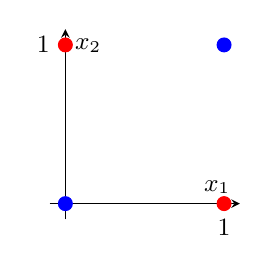
\begin{tikzpicture}
\begin{axis}[
    width=4cm,
    height=4cm,
    xmin=-0.1, xmax=1.1,
    ymin=-0.1, ymax=1.1,
    axis lines=middle,
    xtick={0,1},
    ytick={0,1},
    xlabel={$x_1$},
    ylabel={$x_2$},
    tick label style={font=\small},
    label style={font=\small},
    enlargelimits=false,
    clip=false
]

% Class 0 (blue)
\addplot[
    only marks,
    mark=*,
    mark size=2.5pt,
    blue
]
coordinates {(0,0) (1,1)};

% Class 1 (red)
\addplot[
    only marks,
    mark=*,
    mark size=2.5pt,
    red
]
coordinates {(0,1) (1,0)};

\end{axis}
\end{tikzpicture}
\end{minipage}
\end{center}

A single linear layer has the form
\[
\hat y = w_1 x_1 + w_2 x_2 + b,
\]
which defines a single separating line in $\mathbb{R}^2$.  
XOR is not linearly separable, so no choice of $(w_1,w_2,b)$ can fit all four points.

\bigskip

\textbf{Two–layer ReLU model.}

We now introduce two hidden units with ReLU activation:
\[
\mathrm{ReLU}(z) = \max(0,z).
\]

The network is

\[
\begin{aligned}
z_1 &= w_{11} x_1 + w_{21} x_2 + c_1, \\
z_2 &= w_{12} x_1 + w_{22} x_2 + c_2, \\
h_1 &= \mathrm{ReLU}(z_1), \\
h_2 &= \mathrm{ReLU}(z_2), \\
\hat y &= \alpha h_1 + \beta h_2 + c_3.
\end{aligned}
\]

Choose the parameters (as in the slide):

\[
w_{ij}=1,
\quad
c_1 = 0,
\quad
c_2 = -1,
\quad
(\alpha,\beta) = (1,-2),
\quad
c_3 = 0.
\]

Then

\[
z_1 = x_1 + x_2,
\qquad
z_2 = x_1 + x_2 - 1.
\]

Now evaluate all four inputs.

\[
\begin{array}{c|cccc}
(x_1,x_2) 
& (0,0) & (0,1) & (1,0) & (1,1) \\ \hline
z_1 = x_1+x_2 
& 0 & 1 & 1 & 2 \\[4pt]
z_2 = x_1+x_2-1 
& -1 & 0 & 0 & 1 \\[4pt]
h_1 = \mathrm{ReLU}(z_1) 
& 0 & 1 & 1 & 2 \\[4pt]
h_2 = \mathrm{ReLU}(z_2) 
& 0 & 0 & 0 & 1 \\[4pt]
\hat y = h_1 - 2h_2 
& 0 & 1 & 1 & 0
\end{array}
\]

\bigskip

Thus the network reproduces XOR exactly:
\[
\hat y = y
\quad\text{for all training points.}
\]

\bigskip

\textbf{Why this works.}

Let $s = x_1 + x_2$.  
The hidden layer computes
\[
h_1 = \mathrm{ReLU}(s),
\qquad
h_2 = \mathrm{ReLU}(s-1).
\]

In the diagram below, the dashed line is $s=0$, the solid line is $s=1$, and the shaded band is the region $0 < s \le 1$.  

These two lines partition the plane into three regions:
\[
\quad s \le 0, \quad 0 < s \le 1 \quad s > 1.
\]

\medskip

\noindent
\begin{minipage}[t]{0.55\textwidth}
\vspace{0pt}
\centering
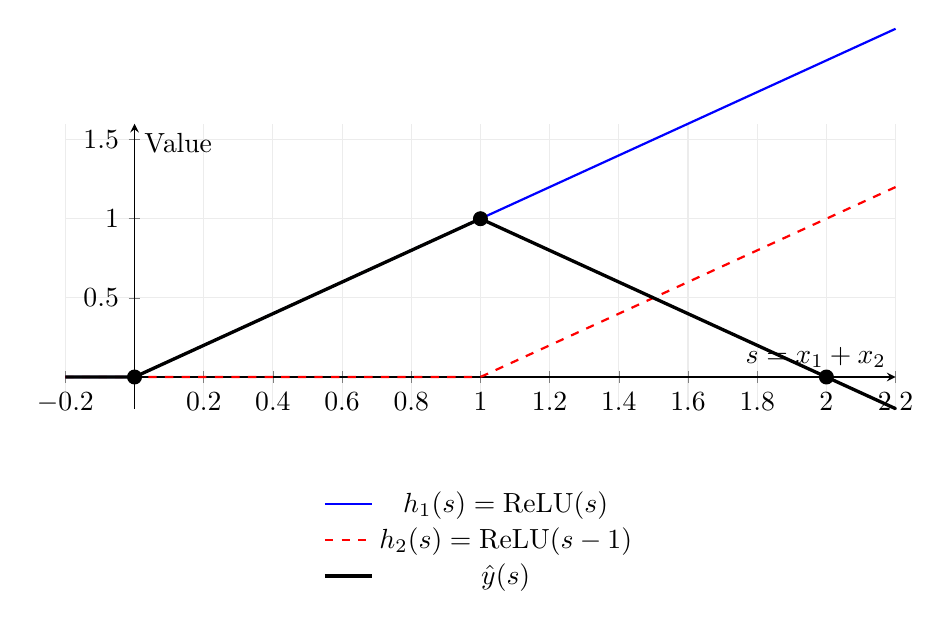
\begin{tikzpicture}
\begin{axis}[
    width=\linewidth,
    height=5.2cm,
    xmin=-0.2, xmax=2.2,
    ymin=-0.2, ymax=1.6,
    axis lines=middle,
    xlabel={$s = x_1 + x_2$},
    ylabel={Value},
    domain=-0.2:2.2,
    samples=300,
    grid=both,
    grid style={gray!15},
    legend style={
        at={(0.5,-0.25)},
        anchor=north,
        draw=none
    },
    clip=false
]

% h1
\addplot[thick, blue]
{max(x,0)};
\addlegendentry{$h_1(s)=\mathrm{ReLU}(s)$}

% h2
\addplot[thick, red, dashed]
{max(x-1,0)};
\addlegendentry{$h_2(s)=\mathrm{ReLU}(s-1)$}

% y
\addplot[very thick, black]
{max(x,0) - 2*max(x-1,0)};
\addlegendentry{$\hat y(s)$}

% XOR points
\addplot[
    only marks,
    mark=*,
    mark size=2.5pt,
    black
]
coordinates {(0,0) (1,1) (2,0)};

\end{axis}
\end{tikzpicture}
\end{minipage}
\hspace{1em}
\begin{minipage}[t]{0.4\textwidth}
\vspace{0pt}

\[
\hat y = h_1 - 2h_2
= \mathrm{ReLU}(s) - 2\,\mathrm{ReLU}(s-1).
\]

\[
\begin{array}{c|c|c|c}
\text{Region} & h_1 & h_2 & \hat y \\ \hline
s \le 0 & 0 & 0 & 0 \\
0 < s \le 1 & s & 0 & s \\
s > 1 & s & s-1 & s - 2(s-1)
\end{array}
\]

\vspace{1em}

On the dataset, $s \in \{0,1,2\}$, so:
\[
\hat y =
\begin{cases}
0 & s=0,\\
1 & s=1,\\
0 & s=2.
\end{cases}
\]

\end{minipage}

\bigskip

The blue curve $h_1(s)=\mathrm{ReLU}(s)$ begins increasing at $s=0$.  
The red dashed curve $h_2(s)=\mathrm{ReLU}(s-1)$ stays flat until $s=1$, then turns on.

The output
\[
\hat y(s)=h_1(s)-2h_2(s)
\]
is the black curve. It rises linearly from $0$ to $1$ as $s$ moves from $0$ to $1$.  
At $s=1$, the second ReLU activates. From that point on, we subtract twice as much as we add, and the function bends downward.

The three dataset values $s=0,1,2$ land exactly at the vertices of this piecewise linear peak, giving outputs $0,1,0$.

\medskip

What matters is the kink at $s=1$.  
A single linear function cannot rise and then turn back down.  
Adding a second ReLU introduces that bend, and that bend is what makes XOR possible.



\newpage
\section{Practice Questions}

\medskip

1. \textit{True or False: A linear layer without bias can always be represented as a matrix multiplication.}

True. A linear layer without bias is exactly a matrix multiplication: $y = Wx$. The output is a vector whose entries are linear combinations of the input features. If a bias term is included, the layer becomes an affine transformation: $y = Wx + b$.

\vspace{1cm}

2. \textit{True or False: A maxpooling layer can always be represented as a matrix multiplication.}

False. Max pooling is a nonlinear operation, so it cannot be represented as a fixed matrix multiplication. In contrast, average pooling is linear and can be represented as a matrix whose rows contain the appropriate averaging weights, e.g., entries equal to $\frac{1}{k}$ over each pooling region size $k$.

\vspace{1cm}

3. \textit{True or False: A common structure for neural networks is 1–4 linear layers (with ReLU activation) followed by 1–4 convolutional layers.}

False. In standard CNN architectures, convolutional layers are applied first to exploit spatial structure and perform feature extraction, often with intermediate pooling. Linear (fully connected) layers are applied afterward for classification. Reversing order would destroy spatial information.


\vspace{1cm}

4. \textit{True or False: A convolutional layer with no bias can always be represented as a matrix multiplication.}

True. A convolutional layer without bias is a linear map, so it can be written as $y = Wx$ for some matrix $W$. This matrix is large, sparse, and highly structured: each row corresponds to one output location, and contains the filter weights placed in the positions corresponding to that local receptive field, with zeros elsewhere. Weight sharing across spatial locations is reflected in repeated patterns within $W$.


\vspace{1cm}

5. \textit{True or False: A fully connected layer is a special case of a convolutional layer.}

True. A fully connected layer can be viewed as a convolution whose kernel has the same spatial dimensions as the input, so it covers the entire input at once and produces a single output per filter.

\vspace{1cm}

6. \textit{True or False: Transfer learning primarily gets its performance from the size of the model.}

False. The benefit of transfer learning comes from pretraining on large, diverse datasets that produce useful feature representations, not from the size of the downstream model. A small model built on top of a pretrained foundation model can perform well because it leverages those learned embeddings.

\vspace{1cm}

7. \textit{True or False: A large model that has been trained on billions of text tokens can be used for transfer learning to image.}

False. A model trained only on text learns representations in a linguistic embedding space and does not learn visual features or spatial structure. Therefore, it cannot be directly used for transfer learning to image tasks without additional multimodal training.

\vspace{1cm}

8. \textit{True or False: If a vision model has been trained on gray scale images, it cannot be used for transfer learning to color images.}

False. A model trained on grayscale images can still learn useful spatial features such as edges, textures, and shapes. These features can transfer to color images, and the model can be fine-tuned to incorporate color-specific information.

\vspace{1cm}

9. \textit{True or False: Minimizing exponential loss is computationally easier than maximizing accuracy (minimizing number of mistakes).}

True. Exponential loss is a smooth, differentiable surrogate loss, so it can be optimized using gradient-based methods. For smooth convex objectives, gradient descent achieves an $\epsilon$-accurate solution in $\mathcal{O}(1/\epsilon)$ iterations. In contrast, accuracy is discontinuous and non-differentiable, making it computationally intractable to optimize directly.

\vspace{1cm}

10. \textit{True or False: Though minimizing exponential loss is easier, it is equivalent to maximizing accuracy.}

False. Exponential loss is a surrogate for 0–1 loss, not an equivalent objective. Minimizing exponential loss does not generally produce the same classifier that maximizes accuracy, since it penalizes misclassified points with large negative margins much more heavily.

\vspace{1cm}

11. \textit{True or False: Gradient descent is guaranteed to find an approximate local minimum of the loss function.}

False. For neural networks, the loss function is non-convex. Gradient descent is not guaranteed to find a local minimum. Under standard smoothness and step-size conditions it converges to a first-order stationary point, which may be a local minimum or a saddle point. If the step size is too large, convergence is not guaranteed.

\vspace{1cm}

12. \textit{True or False: It is generally a good idea to use a smaller step size when using smaller batch size.}

True. Smaller batch sizes produce higher-variance gradient estimates. Using a smaller step size helps stabilize updates and prevents divergence caused by this increased stochastic noise.

\vspace{1cm}

13. \textit{True or False: Though there are no guarantees for non-convex functions, momentum provably improves convergence rate for smooth convex functions.}

True. Momentum dampens movement in oscillatory directions and accelerates movement in consistent directions, improving convergence rate.

\vspace{1cm}

14. \textit{True or False: ADAM is always better than SGD for training deep neural networks.}

False. ADAM often converges faster in early training due to adaptive learning rates, but it does not always achieve better final performance. In many deep learning settings, SGD with momentum can generalize better and produce superior test accuracy.

\vspace{1cm}

15. \textit{True or False: If we do not know what step size to use, taking $\eta = 2^{-t}$ is a good idea.}

False. The schedule $\eta_t = 2^{-t}$ decays exponentially fast, so the total cumulative step size is finite and heavily concentrated in the first few iterations. This makes the method highly sensitive to early noise and generally impractical for optimization.


\vspace{1cm}

16. \textit{True or False: If in a 3-class classification problem the classes are linearly separable, then logistic regression achieves low loss and high accuracy.}

True. Multiclass logistic regression learns linear decision boundaries between classes. If the classes are linearly separable, it can achieve perfect accuracy and arbitrarily low loss.

\vspace{1cm}

17. \textit{Free answer: In a 5-class classification problem in 10 dimensions, logistic regression produces $M, N$-dimensional vectors. What are $M$ and $N$?}

$M = 5$ and $N = 10$. Multiclass logistic regression learns one weight vector per class, each in $\mathbb{R}^{10}$, so the parameter matrix has shape $5 \times 10$.

\vspace{1cm}

18. \textit{Free Response: If the classes are separable, where do those vectors point?}

If the classes are linearly separable, each weight vector points roughly toward the region of feature space where its class resides. The decision boundaries depend on differences between weight vectors, and optimization pushes them in directions that increase separation between class clusters.

\vspace{1cm}

19. \textit{True or False: Just because a CNN achieves high accuracy, it does not necessarily mean that the $(n-1)$st layers produce a near-separable embedding of the data.}

False. If the final layer is a linear classifier (e.g., logistic regression), then the $n-1$ layer must have been linearly separable.

\vspace{1cm}

20. \textit{True or False: If a CNN achieves high accuracy, then for any two classes there is a 2-dimensional embedding where the data points are nearly separable.}

False. High accuracy implies that the learned embedding is approximately linearly separable in its full dimension. However, this does not imply that any pair of classes is separable in a 2-dimensional projection; separability may require higher-dimensional structure.

\vspace{1cm}

21. \textit{True or False: If two words are exact synonyms, Word2Vec produces vectors that are exactly the same.}

False. Word2Vec learns embeddings based on contextual co-occurrence patterns. Even exact synonyms typically appear in slightly different contexts, so their learned vectors will be similar but not exactly identical.

\vspace{1cm}

22. \textit{Free answer: The words ``skibidi'' and ``rizz'' are not in the Word2Vec vocabulary. How would we add them?}

Ideally, we would retrain Word2Vec on a corpus that includes the new words. More realistically, we would continue training the existing model on additional text containing those words so it can learn their embeddings from co-occurrence statistics.

\vspace{1cm}

23. \textit{Free answer: What is a scenario where Recall is the most important metric?}

Recall measures the fraction of actual positive cases that are correctly identified. It is most important when the cost of false negatives is high. A canonical example is medical diagnosis, where failing to detect a disease such as cancer can be far more costly than producing false alarms.

\vspace{1cm}

24. \textit{Free answer: What about NDCG?}

NDCG is a position-sensitive ranking metric that assigns higher weight to relevant items appearing near the top of the ranked list. It is most appropriate when we care about ordering quality, especially placing highly relevant documents at the top, rather than simply retrieving all relevant items.

\vspace{1cm}

25. \textit{Argue for or against: A computationally inexpensive retrieval model should focus on Recall over NDCG.}

For. In a multi-stage retrieval pipeline, a computationally inexpensive first-stage model should prioritize high recall to ensure that most relevant documents are retrieved. A more expensive re-ranking model can then optimize ordering metrics such as NDCG on this smaller candidate set.

\vspace{1cm}

26. \textit{True or False: In Bag of Words, the order of the words does not matter.}

True. Bag of Words represents a document as a vector of word counts and ignores word order. It captures term frequency but does not encode positional information.

\vspace{1cm}

27. \textit{True or False: In contrast, TF.IDF considers the order of the words.}

False. TF-IDF does not encode word order; like Bag of Words, it represents documents as unordered term-frequency vectors. It differs by reweighting terms using inverse document frequency to downweight common words and emphasize more informative ones.

\vspace{1cm}

28. \textit{True or False: TF.IDF is generally better than dense (semantic) embeddings for NDCG, but not for retrieval.}

False. TF-IDF relies on exact term overlap and does not capture semantic similarity, so it often underperforms dense embeddings on ranking metrics such as NDCG when semantic relevance matters. It may achieve high recall for keyword-based queries, but can miss semantically relevant documents that do not share surface terms. Dense embeddings typically improve both semantic recall and ranking quality.

\vspace{1cm}

29. \textit{True or False: TF.IDF is better than Bag of Words because it boosts scientific words.}

True. If scientific terms are less frequent across documents, they will receive higher weight than in a plain Bag of Words representation.

\vspace{1cm}

30. \textit{Free answer: How would you implement TF.IDF and what would the computational cost be?}

We first create a matrix of all zeroes, with dimensions the size of the vocabulary and the number of documents. For each document, we then take the count of each word and divide it by the number of total terms in the document. We create a second vector, 1 by vocabulary size, which has a count for each word of how many documents it appears in (irrespective of how many times it appears in that document), after counting it all up we divide the vector entries by the number of documents. The final output for TF-IDF is the term frequency of a word in its own document multipled by the log of the total documents divided by the number of documents containing the term. The computational cost is The computational cost is $\mathcal{O}(T)$ to compute all term counts over $T$ total tokens, plus $\mathcal{O}(V)$ to compute IDF values for vocabulary size $V$, assuming sparse storage. (Essentially, linear in the size of the corpus). 

\vspace{1cm}

31. \textit{True or False: Since Word2Vec trains on co-occurrence (neighboring words), it is a dense contextual embedding.}

False. Word2Vec produces dense semantic embeddings learned from local co-occurrence statistics, but it is not contextual. Each word has a single fixed vector representation, regardless of the specific sentence in which it appears.

\vspace{1cm}

32. \textit{True or False: BERT as presented in class can be used for question answering, i.e., next word prediction.}

False. BERT is trained with masked language modeling, not autoregressive next-token prediction. It is trained to predict masked tokens within a sentence using full bidirectional context, which makes it effective for learning representations for downstream tasks. Because it is a bidirectional encoder and does not generate tokens sequentially, it cannot directly perform next-word prediction like autoregressive models such as GPT.

\vspace{1cm}

33. \textit{Free answer: What could we do to make BERT usable for next word prediction?}

We would change how BERT is trained so that instead of predicting missing words using both left and right context, it predicts the next word using only the words that come before it. This requires restricting the attention mechanism so each word can only look at earlier words, effectively turning BERT into a left-to-right language model. After predicting a word, we append it to the sequence and repeat the process until an end-of-sequence token is generated.

\vspace{1cm}

34. \textit{True or False: BERT ranks documents (for use in a RAG) by embedding the query as sentence 1 and the document as sentence 2.}

True for a cross-encoder. In a cross-encoder setup, BERT ranks documents by taking as input [CLS] Q [SEP] D [SEP] and producing a relevance score. However, in scalable RAG systems, a bi-encoder is typically used instead, where the query and document are embedded separately and compared via a similarity function.

\vspace{1cm}

35. \textit{True or False: A good RAG should be using a dense embedding but also a sparse embedding like TF.IDF.}

True. A hybrid retrieval approach that combines dense embeddings with sparse methods such as TF-IDF or BM25 can improve performance. Sparse methods capture exact term matches, while dense embeddings capture semantic similarity, and combining them often improves recall and ranking quality.

\vspace{1cm}

36. \textit{True or False: The first step for BERT training is to map tokens to pre-trained embeddings given by a model like Word2Vec.}

False. BERT does not use pre-trained embeddings such as Word2Vec. It learns its own token embeddings from scratch during pretraining, along with positional and segment embeddings.

\vspace{1cm}

37. \textit{True or False: The best way to make BERT a good retriever on our data is to use MLM on our specific dataset.}

False. Masked language modeling adapts BERT to the domain but does not directly optimize retrieval performance. To make BERT a strong retriever, it should be trained with a contrastive or ranking objective using positive and negative query–document pairs.

\vspace{1cm}

38. \textit{True or False: InfoNCE is a version of contrastive learning and essentially uses cross entropy.}

True. InfoNCE is a contrastive learning objective that compares a positive pair against multiple negative pairs using a softmax over similarity scores. It is optimized using cross-entropy loss.

\vspace{1cm}

39. \textit{True or False: InfoNCE can use small batch size, even batch size of 1, but it is not recommended because it will have high variance.}

False. InfoNCE requires negative examples to provide a learning signal. With batch size 1 and no additional negatives, the softmax denominator contains only the positive term, so the loss is always zero regardless of embedding quality. Therefore, meaningful contrastive learning requires multiple negatives.

\vspace{1cm}

40. \textit{True or False: When training a bi-encoder model, we can have overlap in some of the parameters.}

True. In a bi-encoder model, the query and document encoders may share parameters so that both are embedded into the same representation space, although they can also be trained with separate parameters.

\vspace{1cm}

41. \textit{True or False: BERT can be used as a cross-encoder for re-ranking.}

True. BERT can be used as a cross-encoder for re-ranking by taking the input as [CLS] Q [SEP] D [SEP] and producing a relevance score. In practice, this is applied to a small candidate set retrieved by a first-stage retriever, since scoring every document in the corpus would be computationally expensive.

\vspace{1cm}

42. \textit{Describe: How would we turn BERT into a good cross encoder?}

We would fine-tune BERT on labeled query–document pairs using a ranking objective. This could involve supervised relevance labels and optimizing a cross-entropy or pairwise ranking loss so that relevant documents receive higher scores than non-relevant ones.

\vspace{1cm}

43. \textit{Free answer: How else could we generate hard negatives for contrastive learning?}

Hard negatives can be generated by retrieving top-ranked but incorrect documents using a current or weaker retriever and treating them as negatives. Alternatively, we can use in-batch negatives, adversarially perturb relevant documents, or mine negatives from documents that are semantically similar but labeled non-relevant.

\vspace{1cm}

44. \textit{Describe: What is ColBERT and how does it work?}

ColBERT is a late-interaction retrieval model that sits between bi-encoders and cross-encoders. Like a bi-encoder, it encodes queries and documents separately, allowing document representations to be precomputed for efficiency. However, instead of compressing each document into a single vector, it produces contextualized embeddings for each token. At retrieval time, it computes similarity using a MaxSim operation: for each query token, it finds the maximum similarity over all document tokens and sums these scores. This preserves fine-grained token-level interaction while remaining much more efficient than a full cross-encoder.



\vspace{1cm}

45. \textit{True or False: We have been using BERT just as a stand-in and should be exploring other models on HuggingFace.}

True. In practice, we would evaluate multiple transformer models available on HuggingFace, fine-tune them on our task, and compare their performance. Rather than relying solely on BERT, we select the model that achieves the best validation or test performance for our specific retrieval or ranking objective.

\vspace{1cm}

46. \textit{True or False: Fine tuning BERT makes most of its progress in epochs 10–20.}

False. BERT fine-tuning typically achieves most performance gains in the first few epochs. Training for 10–20 epochs often leads to diminishing returns or overfitting, especially on smaller datasets.

\vspace{1cm}

47. \textit{Describe: What does the AutoTokenizer class do and why do we need it?}

AutoTokenizer loads the correct tokenizer associated with a specific pretrained model and converts raw text into model-ready inputs. It handles tokenization, vocabulary lookup, special tokens, padding, truncation, and conversion to input IDs and attention masks. We need it because transformer models operate on token IDs, not raw text, and each model may use a different tokenization scheme.

\vspace{1cm}

48. \textit{Describe: When we download BERT using AutoModelForMaskedLM.from\_pretrained, what do we get back?}

AutoModelForMaskedLM.from\_pretrained returns a pretrained BERT model configured for masked language modeling. This includes the transformer encoder along with a task-specific output head that maps the final hidden states to vocabulary-sized logits for predicting masked tokens. The returned object contains the pretrained weights and is ready for inference or fine-tuning.

\vspace{1cm}

49. \textit{Describe: How could we count the number of parameters in a BERT model?}

We can count the number of parameters by summing the total number of elements in all model parameter tensors. In practice, this can be done by iterating over model.parameters() and summing p.numel() for each parameter. This gives the total number of trainable parameters in the BERT model.

\[
\text{MHSA} =
3 \cdot (hidden\_dim \cdot hidden\_dim + hidden\_dim)
+
(hidden\_dim \cdot hidden\_dim + hidden\_dim)
\]

\[
\text{FFN} =
hidden\_dim \cdot intermediate\_dim + intermediate\_dim
+
intermediate\_dim \cdot hidden\_dim + hidden\_dim
\]

\[
\text{LayerNorm} = 2 \cdot (2 \cdot hidden\_dim)
\]

\[
\text{Total per layer} =
\text{MHSA} + \text{FFN} + \text{LayerNorm}
\]

\[
\text{Total BERT params} =
vocab\_size \cdot hidden\_dim
+
num\_layers \cdot (\text{Total per layer})
\]

\vspace{1cm}

50. \textit{Describe: What is the difference in memory usage between inference and training?}

During inference, we only store model parameters and the activations needed for the forward pass. During training, we must additionally store intermediate activations for backpropagation and the gradients for each parameter. As a result, training requires more memory than inference, about twice more, due to storing activations and optimizer states.

\vspace{1cm}

51. \textit{Describe: How could you use CLIP for searching an image dataset based on a text prompt?}

We would encode all images in the dataset using CLIP’s image encoder and store their embeddings. Given a text prompt, we encode it using CLIP’s text encoder and compute similarity scores (e.g., cosine similarity) between the text embedding and each image embedding. We then rank images by similarity and return the highest-scoring results.

\vspace{1cm}

52. \textit{Describe: How could you use CLIP for zero-shot classification?}

To perform zero-shot classification with CLIP, we first create text prompts describing each class (e.g., "a photo of a cat", "a photo of a dog") and encode them using CLIP’s text encoder. We then encode the input image using CLIP’s image encoder. By computing similarity scores between the image embedding and each class text embedding, we assign the image to the class with the highest similarity, without any task-specific training.

\vspace{1cm}

53. \textit{Describe: How is CLIP trained?}

CLIP is trained with a symmetric contrastive (InfoNCE) loss on batches of image–text pairs. For batch size $N$, we compute similarities

\[
S_{ij} = \frac{\langle t_i, v_j \rangle}{\tau}.
\]

Each text should match only its paired image. The loss is

\[
\mathcal{L}_i^{\text{text}}
=
- \log
\frac{\exp(S_{ii})}
{\sum_{j=1}^{N} \exp(S_{ij})},
\quad
\mathcal{L}_i^{\text{image}}
=
- \log
\frac{\exp(S_{ii})}
{\sum_{j=1}^{N} \exp(S_{ji})}.
\]

The final loss averages both directions. This pulls matched image–text embeddings together and pushes all other batch pairs apart.

\vspace{1cm}

54. \textit{Describe: Why would using BERT to produce multiple tokens at a time be problematic (e.g., feeding in [sentence] [mask] [mask] [mask])?}

Using BERT to predict multiple masked tokens at once is problematic because masked language modeling predicts each masked token independently given the surrounding context. If we input multiple [MASK] tokens, the model does not model dependencies between those predicted tokens. As a result, the generated words may be inconsistent or incoherent, since BERT was not trained to generate sequences autoregressively.

\vspace{1cm}

55. \textit{Describe: If we are producing one token at a time in an autoregressive manner (the way GPT works), what is the difference in computation between using an encoder or a decoder?}

In autoregressive generation, a decoder uses causal masking so each token attends only to previous tokens, and it can cache past key and value states to avoid recomputing attention over the entire sequence at every step. An encoder, which uses bidirectional attention, would require recomputing representations over the full sequence each time a new token is added. Therefore, a decoder is computationally more efficient for autoregressive generation.

\end{document}
